\begin{frame}{Benchmark: Artefacts}
    \begin{columns}[c]
        \begin{column}{0.54\textwidth}
            \begin{itemize}
                \item \textbf{Object Size}\\
                  The size of the artefacts remains mostly unchanged ($\boldsymbol{\pm0.5\%}$)
                \item \textbf{Runtime Performance}\\
                  Change in performance fluctuates\\between $\boldsymbol{\pm1.6\%}$
                \item \textbf{Instruction Frequency}\\
                  \texttt{freeze} instructions represents only the $\boldsymbol{0.04\%-0.06\%}$ of the overall IR instructions
            \end{itemize}
        \end{column}
        \begin{column}{0.44\textwidth}
            \begin{figure}
                \centering
                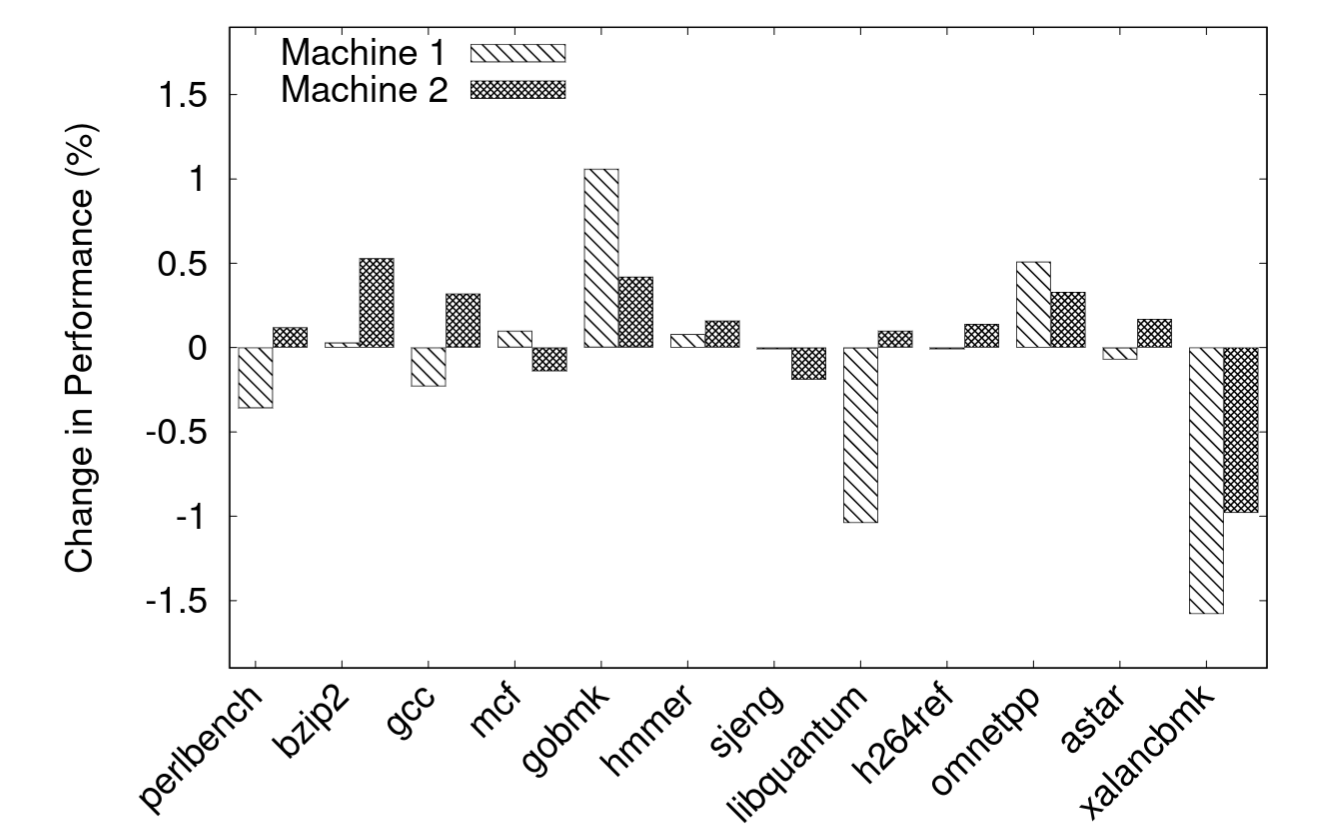
\includegraphics[width=\linewidth]{images/graph.png}
            \end{figure}
        \end{column}
    \end{columns}
    \pdfpcnote{
Object size is essentially unchanged at ±0.5\%. Runtime performance fluctuates
within ±1.6\%, within measurement noise. The key statistic: freeze instructions
represent only 0.04–0.06\% of all IR instructions — the new instruction is rarely
emitted, confirming the low practical overhead. Use the bar chart to ground the
claims visually.
}
\end{frame}
